%!TEX program = xelatex
% 使用 ctexart 文类,UTF-8 编码
\documentclass{article}
  \usepackage{xeCJK,indentfirst}
  \usepackage{amsfonts, amsmath, amssymb}
  \usepackage{graphicx}
  \usepackage[normalem]{ulem}

    \newtheorem{theorem}{Theorem}[section]
  \newtheorem{lemma}{Lemma}  
  \newtheorem{definition}{Definition}[section]
  \newtheorem{proof}{Proof}[section]  
  \numberwithin{equation}{section}

    \newcommand{\bra}[1]{\langle #1 |}
  \newcommand{\ket}[1]{| #1 \rangle}
  \newcommand{\bracket}[2]{\langle #1 | #2 \rangle}
  \newcommand{\bracketl}[3]{\langle #1 | #2 | #3 \rangle}
  \newcommand{\func}{\mathrm \,}
  \newcommand{\define}[2]{
   \begin{definition}
    \begin{description}
    \item[#1]
    #2
   \end{description}
   \end{definition}
  }
  \newcommand{\mean}[1]{\langle #1 \rangle}

  \newcommand{\sch}{Schr\"odinger} 
  \newcommand{\grad}{\nabla}

  \setlength{\parindent}{2em}
  \setlength{\textheight}{240mm}
  \setlength{\textwidth}{155mm}
  \setlength{\oddsidemargin}{0mm}
  \setlength{\evensidemargin}{0mm}
  \setlength{\topmargin}{-20mm}
  \renewcommand{\baselinestretch}{1.2}
  \title{王林军老师课题组本科生入门指南}
  \author{Chaoqun ZHANG-张超群\\Rui LI - 李睿}
  \date{\today}
  \begin{document}
    \maketitle
    \tableofcontents
    \newpage
    \section{引言}
  \begin{quote}
    老师说``这个东西很简单''的时候,往往是普通化学本科生搞不定的东西。
    \begin{flushright}
      ————李睿,在抱怨化学本科生编程能力不够时的调侃
    \end{flushright}
  \end{quote}
  \begin{quote}
    你有问题就要问,你如果不问,我就默认你都会了。
    \begin{flushright}
      ————王林军老师
    \end{flushright}
  \end{quote}

  欢迎进入王林军老师的课题组!无论您是由于何种原因,出于什么目的,来到王林军老师的课题组足以证明了您的勇气!\sout{看,在王林军老师组的都很休闲的}

  由于王林军老师研究比较``底层''的计算化学,所以会对数学、物理、计算机等知识内容会有更高的要求。而历届在王老师做事的本科生们都不止一次地抱怨来王老师的课题组的门槛非常高,而且没有合适的入门指南,使得难度进一步提高(\sout{你会发现你听了一年组会都学不到什么东西}),同时化学系对数理方面的要求实在不敢恭维,从而刚参加王老师的组会的时候会近乎100\%地出现``这是什么/我是谁/我在干什么''的疑惑,因此编者们共同商量,觉得出一份入门指南非常的重要,于是草草编写了这样的一份。

    \section{Linux基础及服务器使用}
    Linux和macOS、Windows并称为三大电脑操作系统,都是用来完成用户和计算机之间的互动。Linux由于其出色的稳定性以及免费(相对于Unix系统),被广泛用于服务器的操作系统。当然Linux是存在图形界面的,但它的最为使用,也最为核心的部分还是它的终端,也就是字符界面。为了如何操作这玩意儿,一些基础知识是必须的。

    \subsection{连接至服务器}
    王林军老师课题组是使用浙大西溪校区的超级计算机集群来进行日常的工作的,简单地就叫服务器。听起来非常高大上,我们所编写的程序(或者商业软件)在普通计算机上当然也可以运行,只是很多时候
    需要过分长的时间,还要保持电脑全天开机,基本是不可能的,因此我们需要交给集群处理。

    集群计算机的操作系统都是Linux系统,我们需要用自己的个人电脑连接到服务器上,这样可以实现对服务器的远程操作,如果你的个人电脑是Linux或者mac系统,可以直接
    在终端使用ssh命令登录服务器,但是由于组内工作电脑和多数个人电脑为Windows系统,这一部分我们暂时不作展开,有兴趣的同学可以直接网上搜索。在Windows系统下连接
    Linux服务器,需要通过一些软件的辅助,比如PuTTY和XSHELL,鉴于后者有不少优势,比如更加新人友好\sout{并且好看},我们就以后者举例。

    XSHELL目前有官方的中文网站\footnote{https://www.netsarang.com/zh/xshell/},可以找到学生用的免费版,下载XSHELL和XFTP两个软件,
    前者是一个在Windows操作系统下实现ssh功能的软件,用于连接远程服务器;后者是实现sftp功能的软件,用于服务器和本地计算机之间的文件传递。
    这两个软件可以满足在理论计算化学组连接远程服务器的一切需求。安装好之后打开XSHELL,如下图所示新建会话,
    \begin{center}
      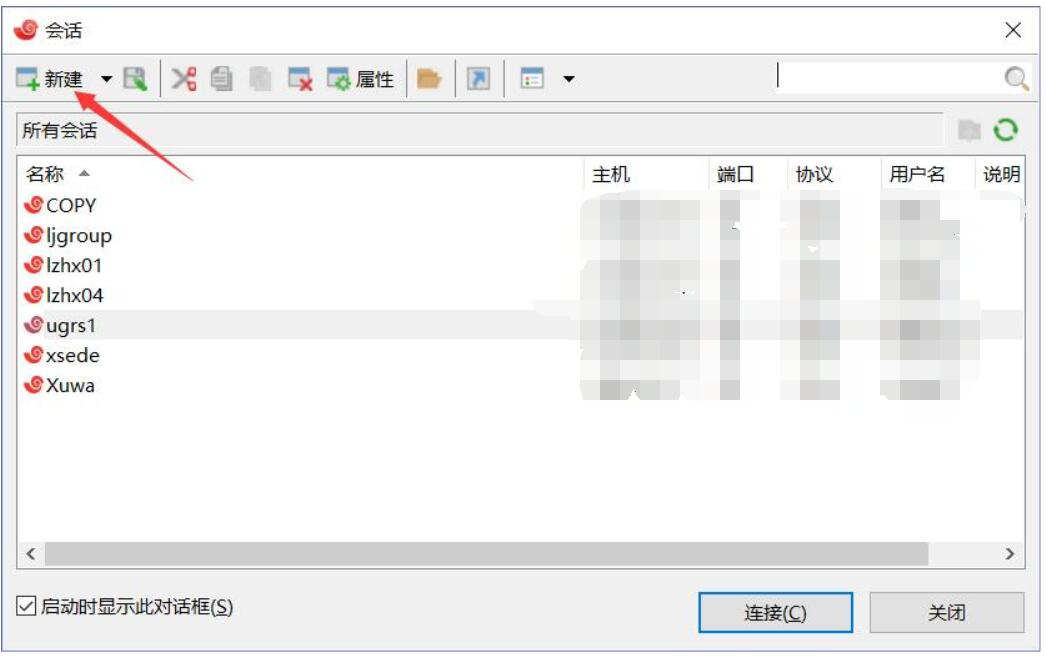
\includegraphics[width = 14cm]{fig/xshell1.png}
    \end{center}
    其中主机填入10.22.51.200

    \subsection{Linux基本操作}
    \begin{description}
    \item[cd]
      进入输入目录的文件夹;
      `cd folder/'
      P.S : `cd ..' 返回上一级文件夹
    \item[ls]
      列出所在文件夹的子文件夹;

    \item[vi / vim]
      打开文件查看内容;vim事实上是一个文本编辑器(比方说这个文档的一部分也是用vim编辑的)

      P.S :输入不存在的文件可直接创立该文件;

    vim有一个梗,就是几乎所有的人刚上手的时候都不知道{\textbf 该怎么退出}。在这里面稍微描述一下最基本的使用方法:
    \begin{description}
      \item[i / Ins] 如果已经打开了某个文本,那么这两个键中的一个能够允许你对文本作出修改。它左下角会显示 ``--INSERT--'' 这样的文段,这说明你处在编辑模式,这时候你按出的大部分操作会如同你使用大部分文本编辑器的时候一样,会完整地呈现在你正在修改的文本上。
      \item[Esc] 无论你处在何种模式,按了Esc你就能回到正常模式,在该模式下你可以用它自身的快捷键来直接作出一些修改,也可输入命令来完成别的操作(比如{\textbf 退出})。

      \item[:q!] 这里`:'表示进行对vim程序自身的命令,`q'是quit,`!'表示强制。也就是输了这个命令并按回车后会强制退出并不保存文件。

      \item[:wq] 以此类推,这个表示的是保存并退出。没错,`:w'就是进行保存,并不退出。
    \end{description}
    好了,现在你也是会用vim的人了!跟我一起喊,\sout{vim天下第一!}
    \item[pwd]
      显示所在目录路径;它会显示所处目录的绝对路径,而这个绝对路径是你在任何别的目录下都能访问的。从该角度出发,事实上别的几乎所有操作都可以指定绝对路径(比如简单的访问,或者复制,或者在程序里面调用/生成文件)。

    \item[mkdir]
      在所在目录下建立文件夹:
      `mkdir levest' 表示建立名字为`levest'的文件夹

    \item[cp] 复制文件至某个目录
      `cp einfield.com slot' 表示将`einfield.com' 在`slot'文件夹下进行粘贴

    \item[mv] 原则上它表示将某个东西移动到什么地方,但它的另一个神奇操作在于它可以重命名文件/文件夹(后缀还是要加好)。

    \item[rm] \textbf{ 危险!}这是表示删除操作。

    \item[-r] 在Linux中大部分的`-*' 表示了所进行的主要命令的附加指令(附加属性,\sout{buff})。像这里`-r'一般用来表示是对整个文件夹进行操作,像上面的cp, rm 都可以加上-r。

    \item[*] *一般在Linux表示缺省符号,也就是在这里面可以填任何东西。比方说,`rm *.c' 表示任何后缀为`.c'的文件都会被删除\footnote{这就是为什么sudo rm -rf /* 这个梗会流行的原因。}。

  \end{description}

    \section{数学基础}
    \subsection{符号使用}
    在量子力学相关领域,人们使用``左矢''(bra)和``右矢''(ket)来描述一个``状态''。我们可以先简单地认为右矢代表了一个列向量,左矢则代表了一个行向量。它们是这么表示的:
    \[
    | \xi \rangle \rightarrow \text{右矢}, \langle \xi | \rightarrow \text{左矢}    
    .\]  
    我们知道,一个行向量和列向量相乘能够得到一个实数,这也可以理解为两个行向量进行内积的过程,比如两个右矢$| \xi_1 \rangle $ 和$| \xi_2 \rangle $ ,此时它表示为
    \[
    \langle \xi_1 | \xi_2 \rangle 
    .\] 
    当然量子力学远不止于此,它有可能包括了各种奇奇怪怪的东西,使得它并不能完全用向量来描述,比如在线性代数里我们有时候需要用矩阵,在量子力学里它们统统被概括为算符。算符是作用在矢量上的。如果你学过张量分析/矢量代数,你还可以认为它代表了一个张量。有些人们喜欢用$\hat{Q}$类似这样的形式来表达一个算符(也就是加个帽子),也有些人喜欢用粗体,比如$\mathbf{Q}$这样来表达,也有人不加任何东西\footnote{没错就是发明这一套符号系统的\Large{Dirac}大佬。},只要它``在该在的地方''就可以识别为一个算符。算符放在左矢的右边,或者右矢的左边,或者左矢和右矢的中间,也就是
    \[
    \hat{Q}| \xi \rangle ,\langle \xi | \hat{Q}, \langle \xi_1 | \hat{Q} | \xi_2 \rangle   
    .\] 
    到了这里,当然就会出现作用顺序(方向)的问题。不过其实这一套和线性代数非常相像\footnote{事实上这一套就是线性代数——也就是海森堡开发的矩阵力学的核心,量子力学就是线性代数(并不是)},算符默认是作用在右边的,如果需要作用在左矢,那么对应的算符为原算符的厄米共轭(Hermite Conjugate),用$\hat{Q}^\dagger$来表达。那么某种程度上,左矢代表的是右矢的共轭转置,左矢和右矢相作用得到的是两者的内积。

    当然这么说可能很难有感觉这些到底是什么东西,让我们再换一种方式来表达。算符,变换,这些东西实则上都代表了类似于函数的概念,也就是传进去一个东西,传出去另一个东西,这两个东西可以相等,可以完全不是同一类。而左矢和右矢则代表了可以传进去的``参量'',并经过算符作用后得到了另一个左矢或右矢。比如一个关于$x$的函数$f(x)$,经过求导算符$\frac{d }{d x} $作用后得到它的导函数$f'(x)$,实则上也没有脱离这样的描述体系\footnote{从而为Dirac说明海森堡的矩阵力学和薛定谔的波动力学是等价表述做好了铺垫。}。

    \subsection{傅立叶变换}
  \begin{quote}
    它,改变了世界。
    \begin{flushright}
      ——李睿,谈傅立叶变换时
    \end{flushright}
  \end{quote}     
  咕咕……咕咕咕……

    \section{量子力学}

    \begin{enumerate}
    \item 算符对易子:
  \begin{equation}
  [A,B] = AB - BA
  \end{equation}

  \item 算符对易常用公式:
  \begin{align}
  [A,BC]& = [A,B]C - B[A,C]\\
  [AB,C]& = [A,C]B + A[B,C]
  \end{align}

  \item $x$与$p$的对易关系:
  \begin{equation}
  [x,p]\psi=(xp-px)\psi = -i\hbar[x \frac{\partial}{\partial x}\psi-\frac{\partial}{\partial x}(x\psi)]= i\hbar \psi
  \end{equation}

  \item 波函数是量子态在基组中的投影:
  \begin{equation}
  \psi (x) = \langle x | \psi \rangle , \quad \psi(p) = \langle p | \psi \rangle
  \end{equation} 
\end{enumerate}
  

\begin{theorem}
Ehrenfest Theorem:

\begin{align}
\mean{\textbf{p}}= m \frac{d \mean{\textbf{x}}}{dt}\\
\mean{\textbf{F}}= \frac{d\mean{\textbf{p}}}{dt}
\end{align}
\end{theorem}

\begin{proof}
  充分考虑到
  \begin{equation}
  \frac{d\ket{\phi}}{dt}=\frac{1}{i\hbar}[\frac{\textbf{p}^2}{2m}+V(\textbf{x})]\ket{\phi}
  \end{equation}

  \begin{align*}
  \frac{d \mean{\textbf{x}}}{dt}  & = \frac{d \bracketl{\psi}{\textbf{x}}{\psi}}{dt} \\ 
  & = \frac{d\bra{\psi}}{dt} \textbf{x} \ket{\psi} + \bra{\psi} \textbf{x} \frac{d\ket{\psi}}{dt} \\
  &= - \frac{1}{i \hbar}\bra{\psi}[\frac{\textbf{p}^2}{2m}+V(\textbf{x})]\textbf{x}\ket{\psi}+ \bra{\psi}\textbf{x}\frac{1}{i\hbar}[\frac{\textbf{p}^2}{2m}+V(\textbf{x})]\ket{\psi}\\
  &= -\frac{1}{i\hbar}(\frac{\textbf{p}^2}{2m}\textbf{x}-\textbf{x}\frac{\textbf{p}^2}{2m})\ket{\psi}\\
  &= -\frac{1}{2mi\hbar}\bracketl{\psi}{[\textbf{p}^2,\textbf{x}]}{\psi}\\
  &=-\frac{1}{2mi\hbar}\bracketl{\psi}{2\textbf{p}[\textbf{p},\textbf{x}]}{\psi}\\
  &=\frac{1}{m}\bracketl{\phi}{\textbf{p}}{\phi}\\
  &=\mean{\textbf{p}}
  \end{align*}

  \begin{align*}
  \frac{d\mean{\textbf{p}}}{dt} &= \frac{d\bracketl{\psi}{\textbf{p}}{\psi}}{dt}\\
  &=\frac{d\bra{\psi}}{dt} \textbf{p} \ket{\psi} + \bra{\psi} \textbf{p} \frac{d\ket{\psi}}{dt} \\
  &= - \frac{1}{i \hbar}\bra{\psi}[\frac{\textbf{p}^2}{2m}+V(\textbf{x})]\textbf{p}\ket{\psi}+ \bra{\psi}\textbf{p}\frac{1}{i\hbar}[\frac{\textbf{p}^2}{2m}+V(\textbf{x})]\ket{\psi}\\
  &= -\frac{1}{i\hbar}\bracketl{\psi}{[V(\textbf{x}),\textbf{p}]}{\phi} \\
  & = -\frac{1}{i\hbar}\bracketl{\phi}{i\hbar\frac{\partial V(\textbf{x})}{\partial \textbf{x}}}{\phi}\\
  & = \bracketl{\phi}{[-\frac{\partial V(\textbf{x})}{\partial \textbf{x}}]}{\phi}\\
  & = \mean{\textbf{F}}
  \end{align*}

  \begin{align*}
  [V(\textbf{x}),\textbf{p}] \ket{\psi} & = [V(x),-i\hbar \frac{\partial}{\partial \textbf{x}}]\ket{\psi}\\
  & = -i\hbar V(x) \frac{\partial }{\partial \textbf{x}} + i\hbar \frac{\partial}{\partial \textbf{x}}[V(\textbf{x})\ket{\psi}]\\
  &= -i\hbar V(x) \frac{\partial }{\partial \textbf{x}}+ i\hbar \frac{\partial V(\textbf{x})}{\partial \textbf{x}}\ket{\psi} + i\hbar V(\textbf{x}) \frac{\partial \ket{\psi}}{\partial \textbf{x}}\\
  &= i\hbar \frac{\partial V(\textbf{x})}{\partial \textbf{x}} \ket{\psi}
  \end{align*}
  \end{proof}
    \section{量子化学-电子结构基础}

    \section{非绝热动力学与势间跳跃方法}
    在Born-Oppenheimer近似下,我们可以针对特定的分子构型(核的位置)计算对应的电子能量,对于不同的核坐标$\mathbf{R}$(习惯上大写
    表示原子核坐标,小写表示电子坐标),可以给出一系列电子能量$U=U(\mathbf{R})$,这就是我们通常所说的势能面。需要注意的是,
    势能面是基于BO近似的结果,这是一切的前提。
    
    (TODO需要修改)BO近似几乎是量子化学中最重要的近似条件,可以适用于我们平常遇到几乎全部静态问题和很多动态问题,BO近似下基态的势能面也是比较合理的。
    但是在一些情况下,尤其是当研究的体系涉及多个激发态——比如光激发然后通过非辐射方式回到基态过程时,BO近似就显示出了其弊端。一类
    常见的BO近似失效的情景称为圆锥交叉(conical intersections),理想的圆锥交叉指的是两个势能面的至少两个维度在某一分子构型上简并(交叉)。
    通过早期实验光谱上和理论上的研究,人们发现涉及圆锥交叉的势能面的动力学是BO近似无法描述的。
    
    为了解决这个问题,必须把原子核和电子的运动一起加进动力学模拟的过程中,这类动力学通常称为非绝热动力学(non-adiabatic coupling)。处理核的运动
    有多种方式,经典的分子动力学就是只有原子核的运动,不属于非绝热动力学的范畴,但是经典运动是处理原子核的一种方式,另外还可以将原子核的运动
    也用量子力学求解,进行全量子的非绝热动力学模拟。王林军老师课题组常用的势间跳跃(surface hopping)方法,就是原子核做经典处理,电子做量子处理
    的一种混合量子经典的非绝热动力学方法。
      \subsection{非绝热耦合}
        作为“动力学”下的讨论,我们一定会用到含时Schr\"odinger方程:
        \begin{equation}
          i \hbar \frac{\mathrm{d} | \psi \rangle}{\mathrm{d} t}=\hat{H} | \psi \rangle
        \end{equation}
        或者是与之等价的量子Liouville方程:
        \begin{equation}
          \frac{\mathrm{d} \hat{\rho}}{\mathrm{d} t}=\frac{-i}{\hbar}[\hat{H}, \hat{\rho}]
        \end{equation}
        Liouville方程的优点是直接演化密度矩阵(TODO电子结构部分解释),动力学所关心的问题就是波函数/密度矩阵如何随时间演化,而在一般的量子力学
        语境中,波函数的演化通常是波函数系数的演化,含时的波函数可以写作不含时基组的线性组合
        \begin{equation}
          |\psi(\mathbf{r}, \mathbf{R}, t)\rangle=\sum_{j} c_{j}(t) |\phi_{j}(\mathbf{r} ; \mathbf{R})\rangle
        \end{equation}
        这个不含时基组可以是(也可以不是)定态Schr\"odinger方程的解,我们讨论一个更一般的情况,这个基组只被要求满足正交归一性,
        带入含时Schr\"odinger方程得到
        \begin{equation}
          \sum_j c_j \hat{H}|\phi_j\rangle=i \hbar \frac{\mathrm{d} | \psi \rangle}{\mathrm{d} t}=i \hbar\sum_j\left(\dot{c}_j|\phi_j\rangle+c_j\frac{\mathrm{d}}{\mathrm{d}\mathbf{R}}|\phi_j\rangle\dot{\mathbf{R}}\right)
        \end{equation}
        在上式左右两端乘以$\langle\phi_i|$就得到了
        \begin{equation}
          i \hbar \dot{c}_{i}=\sum_{j} c_{j}\left(V_{i j}-i \hbar \dot{R} \cdot d_{i j}\right)
          \label{ihcdot}
        \end{equation}
        其中定义了$V_{ij}=\langle\phi_i|\hat{H}|\phi_j\rangle$和$d_{ij}=\langle\phi_i|\frac{\mathrm{d}}{\mathrm{d}\mathbf{R}}|\phi_j\rangle$,
        后者称为非绝热耦合(non-adiabatic coupling,NAC),该项所引发的问题是非绝热动力学的领域核心问题之一。在这里,我们可以通过另一种方式来理解它
        名字的来源以及它的物理意义:如果我们用最简单的数值方法计算非绝热耦合,即
        \begin{equation}
          d_{ij}=\langle\phi_i|\frac{\mathrm{d}}{\mathrm{d}\mathbf{R}}|\phi_j\rangle\approx\langle\phi_i(\mathbf{R})|\frac{|\phi_j(\mathbf{R}+\Delta\mathbf{R})\rangle-|\phi_j(\mathbf{R})\rangle}{\Delta\mathbf{R}}
          =\frac{\langle\phi_i(\mathbf{R})|\phi_j(\mathbf{R}+\Delta\mathbf{R})\rangle}{\Delta\mathbf{R}}
        \end{equation}
        上式的最后结果说明非绝热耦合直接正比于不同核位置的波函数之间重叠,要知道如果这些态在同一个
        核坐标下满足正交性,当$i\neq j$时不应该有重叠。之所以有不等于0的非绝热耦合,就是因为在不同核坐标下的不同电子态间有“耦合”,
        而这个耦合正是超越BO近似所引入的,是“非绝热”而引入的。
        
        最后,尽管计算非绝热耦合在很多时候都非常重要,我们在这篇向导中不作特别仔细的讨论,通常有类似上式的数值求解方法
        和通过解析导数的方法求解,但是具体要在不同表象下讨论,下一小节我们就要介绍所谓绝热表象与透热表象。
      \subsection{绝热表象与透热表象}
        本文中所说的绝热(adiabatic)与透热(diabatic)与热学中相关概念并无直接联系,属于量化领域常用的一种表达。
        绝热是基于Born–Oppenheimer近似而言的,需要注意由于翻译的问题,请不要混淆非绝热(non-adiabatic)和透热(diabatic)
        两个概念。

        根据Troy Van Voorhis在他那篇著名的综述\footnote{Annu. Rev. Phys. Chem. 2010. 61:149–170: The Diabatic Picture of Electron Transfer, Reaction Barriers, and Molecular Dynamics}
        中的说法,绝热态定义为BO近似下的哈密顿量的本征态,也就是说在BO近似下解定态Schr\"odinger方程(电子结构计算)得到的波函数就是
        绝热态,即$\hat{H}|\phi_i\rangle=E_i|\phi_i\rangle$。而透热态是指不随核坐标(分子构型)变化的态,最常用的
        就是Troy提到的NaCl的例子,透热态其实是量子化学家们为了理解图像和计算的方便提出的不真实存在的量子态,如不管
        Na和Cl的距离多大,永远为两个中性原子的态,或者是永远是两个离子的态。这样说来十分抽象,但是本质上就是
        其波函数不随核坐标变化而变化,一个严格的定义为透热态的非绝热耦合为0(甚至很多时候简化为$\frac{\mathrm{d}}{\mathrm{d}\mathbf{R}}|\phi_j\rangle=0$)。
        在电荷转移中的图像更加清晰,如果电荷转移发生在两个分子间,透热态通常定为电荷局域在第一个分子上的态和局域在第二个分子上的态,
        而真实的态(电荷分散在两个分子上,也就是绝热态)是两个透热态的线性组合。

        在实际操作中,绝热态是很容易得到的,因为绝热态是哈密顿量本征态,我们可以用各种电子结构的计算方法得到他们,但是
        在绝热表象下,两个绝热态之间存在非绝热耦合,势能面间也会有圆锥交叉或者trivial crossing,这几项往往会给动力学计算带来
        很大难度,因此人们很多时候会希望通过绝热态的线性组合来构建透热态,在透热表象下进行动力学模拟,这个过程称为透热化(diabatization)。透热化的
        方法非常多,本向导中也不作仔细的展开,但是根据Troy的综述,真正的透热态是难以通过绝热态线性组合得到的,所以很多文章中会使用
        构建半透热态(quasi-diabatic state)的说法。需要注意,根据非绝热耦合等于零的定义,透热态按照某个固定的系数的线性组合还是透热态,也就是
        透热态并不是唯一的,这种不唯一性给了量子化学家构建透热态的更大的自由度。这也是目前透热化的方法多种多样的一个原因。

        在透热表象下,由于透热态不是哈密顿量的本征态,所以此时哈密顿量不再是对角矩阵,而是有非零的非对角元,在某些问题(如电荷转移)中,
        这些非对角元通常被叫做转移积分(transfer integrals),对角化透热态哈密顿量应该能重新得到绝热态的能量。
        在透热表象下,可以认为式(\ref{ihcdot})中的$V_{ij}$就是转移积分,所以在某种程度上说,即使透热化并不完全,仍有很小数值的
        非绝热耦合,只要该项对转移积分是一个小量,对动力学的影响也可以忽略,但是在绝热表象中由于$V_{ij}=0$,因此
        非绝热耦合即使有些时候较小,仍是十分重要的。
      \subsection{势间跳跃方法与FSSH}
  \end{document} 

